\documentclass[11pt]{article}
\usepackage{tikz}
\usepackage{amssymb}
\usepackage{geometry}
\geometry{letterpaper, landscape, margin=0.4in}
\usetikzlibrary{positioning, calc}

% Door macros
\newcommand{\hdoor}[2]{%
  \fill[white,draw=black,thick] ({#1-0.1},{#2-0.12}) rectangle ({#1+0.1},{#2+0.12});%
}
\newcommand{\vdoor}[2]{%
  \fill[white,draw=black,thick] ({#1-0.12},{#2-0.1}) rectangle ({#1+0.12},{#2+0.1});%
}

\begin{document}

\begin{center}
{\Huge \textbf{The Grain Mother's Ruin}}\\[0.3em]
{\Large Level 3B --- The Silo Depths | 10 Keyed Areas}
\end{center}

\vspace{0.3em}

\begin{center}
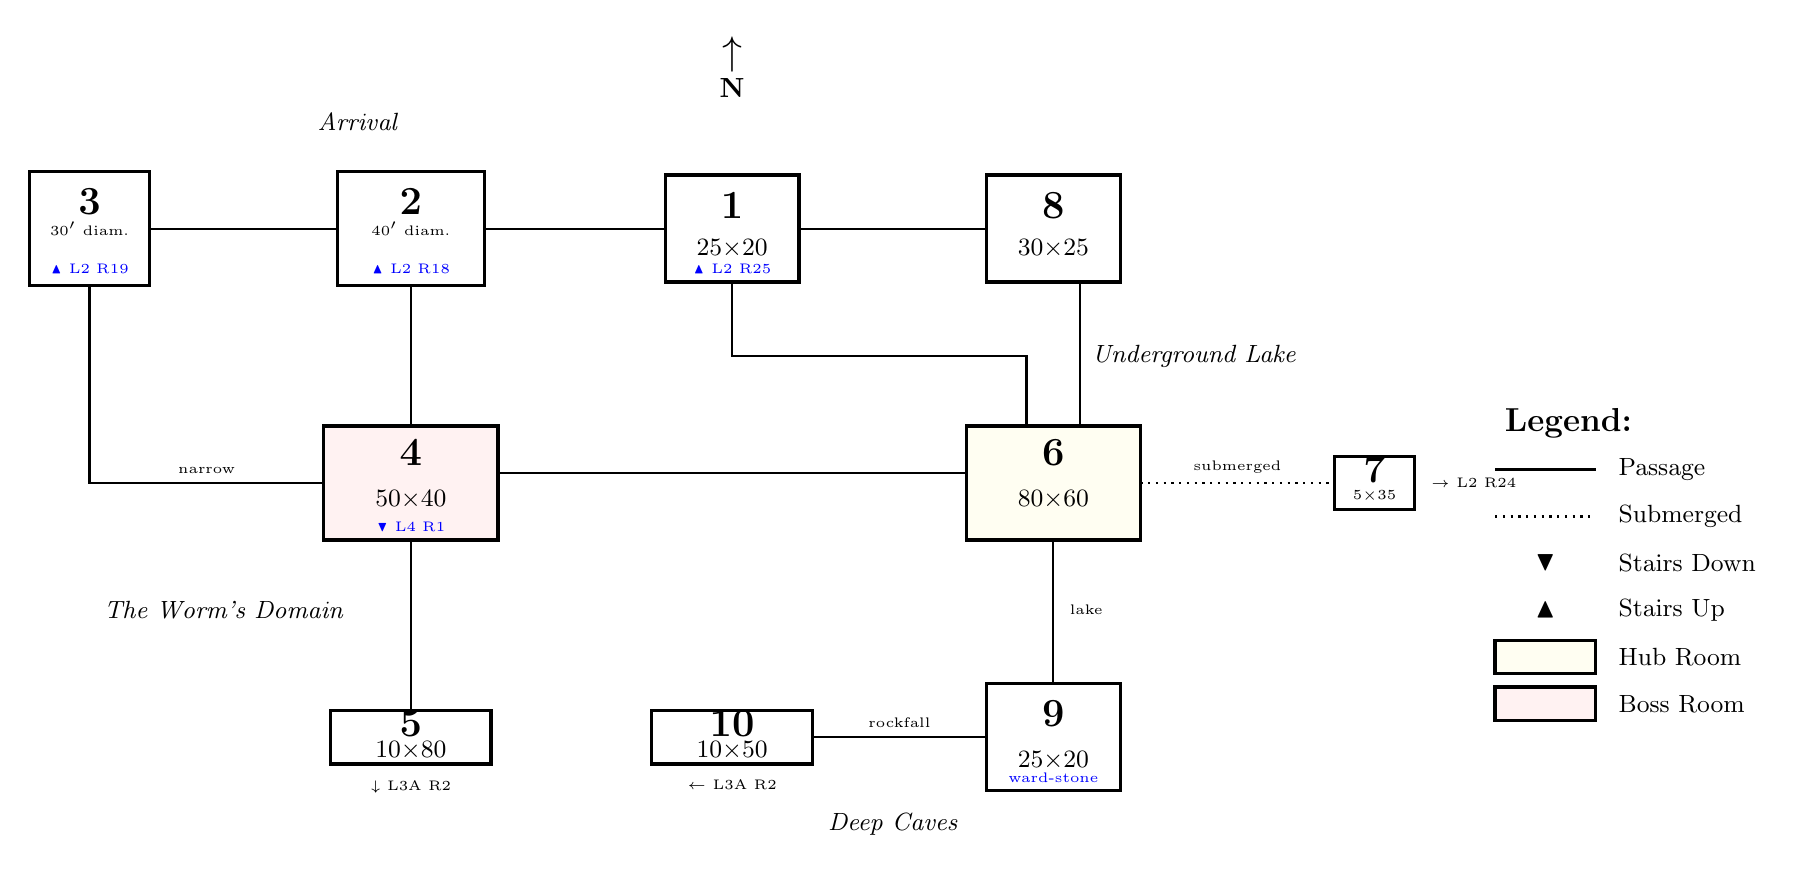
\begin{tikzpicture}[
    room/.style={draw, very thick, rectangle},
    hub/.style={draw, very thick, rectangle, fill=yellow!5},
    boss/.style={draw, very thick, rectangle, fill=red!5},
    connection/.style={draw, thick},
    secret/.style={dashed, thick},
    trap/.style={red},
    scale=0.85
]

% ============================================================
% GRID PARAMETERS
% CellW=3.0, CellH=2.0, Gutter=1.8
% Cols: c0(x=1.5) c1(x=6.3) c2(x=11.1) c3(x=15.9) c4(x=20.7)
% Rows: r1(y=4.8) r2(y=8.6) r3(y=12.4)
% Vertical gutters: c0-c1(x=3.9) c1-c2(x=8.7) c2-c3(x=13.5) c3-c4(x=18.3)
% Horizontal gutters: r1-r2(y=6.7) r2-r3(y=10.5)
% ============================================================

% ============================================================
% NORTH ARROW
% ============================================================
\node at (11.1, 15.0) {\Large $\uparrow$};
\node at (11.1, 14.5) {\textbf{N}};

% ============================================================
% ZONE: Arrival (Rooms 1-3)
% Grid region: r3
% ============================================================

% Room 1: The Bone Stair Landing (25x20 ft, irregular)
% Cell: (c2, r3) -> center (11.1, 12.4)
% Rect: (10.1, 11.6) to (12.1, 13.2)
\draw[room] (10.1,11.6) rectangle (12.1,13.2);
\node at (11.1,12.75) {\Large \textbf{1}};
\node[font=\small] at (11.1,12.1) {25$\times$20};
\node[blue,font=\tiny] at (11.1,11.8) {$\blacktriangle$ L2 R25};

% Room 2: The Grain Chute (40' diameter, circular)
% Cell: (c1, r3) -> center (6.3, 12.4)
% Rect: (5.2, 11.55) to (7.4, 13.25)
\draw[room] (5.2,11.55) rectangle (7.4,13.25);
\node at (6.3,12.8) {\Large \textbf{2}};
\node[font=\tiny] at (6.3,12.4) {40$'$ diam.};
\node[blue,font=\tiny] at (6.3,11.8) {$\blacktriangle$ L2 R18};

% Room 3: The East Shaft Floor (30' diameter, circular)
% Cell: (c0, r3) -> center (1.5, 12.4)
% Rect: (0.6, 11.55) to (2.4, 13.25)
\draw[room] (0.6,11.55) rectangle (2.4,13.25);
\node at (1.5,12.8) {\Large \textbf{3}};
\node[font=\tiny] at (1.5,12.4) {30$'$ diam.};
\node[blue,font=\tiny] at (1.5,11.8) {$\blacktriangle$ L2 R19};

% ============================================================
% ZONE: The Worm's Domain (Rooms 4-5)
% Grid region: r2 (R4), r1 (R5)
% ============================================================

% Room 4: The Worm Den (50x40 ft, irregular) -- BOSS: Illaktamus's lair
% Cell: (c1, r2) -> center (6.3, 8.6)
% Rect: (5.0, 7.75) to (7.6, 9.45)
\draw[boss] (5.0,7.75) rectangle (7.6,9.45);
\node at (6.3,9.05) {\Large \textbf{4}};
\node[font=\small] at (6.3,8.35) {50$\times$40};
\node[blue,font=\tiny] at (6.3,7.95) {$\blacktriangledown$ L4 R1};

% Room 5: The Acid-Bored Tunnel (10x80 ft)
% Cell: (c1, r1) -> center (6.3, 4.8)
% Rect: (5.1, 4.4) to (7.5, 5.2)
\draw[room] (5.1,4.4) rectangle (7.5,5.2);
\node at (6.3,5.0) {\Large \textbf{5}};
\node[font=\small] at (6.3,4.6) {10$\times$80};

% Level 3A connection annotation for Room 5
\node[font=\tiny,anchor=north] at (6.3,4.3) {$\downarrow$ L3A R2};

% ============================================================
% ZONE: The Underground Lake (Rooms 6-7)
% Grid region: r2
% ============================================================

% Room 6: The Lakeshore Cavern (80x60 ft, irregular) -- HUB: most connections
% Cell: (c3, r2) -> center (15.9, 8.6)
% Rect: (14.6, 7.75) to (17.2, 9.45)
\draw[hub] (14.6,7.75) rectangle (17.2,9.45);
\node at (15.9,9.05) {\Large \textbf{6}};
\node[font=\small] at (15.9,8.35) {80$\times$60};

% Room 7: The Drowned Passage (5x35 ft, submerged tunnel)
% Cell: (c4, r2) -> center (20.7, 8.6)
% Rect: (20.1, 8.2) to (21.3, 9.0)
\draw[room] (20.1,8.2) rectangle (21.3,9.0);
\node at (20.7,8.8) {\Large \textbf{7}};
\node[font=\tiny] at (20.7,8.4) {5$\times$35};

% Level 2 connection annotation for Room 7
\node[font=\tiny,anchor=west] at (21.4,8.6) {$\rightarrow$ L2 R24};

% ============================================================
% ZONE: The Deep Caves (Rooms 8-10)
% Grid region: r3 (R8), r1 (R9, R10)
% ============================================================

% Room 8: The Fungal Grotto (30x25 ft)
% Cell: (c3, r3) -> center (15.9, 12.4)
% Rect: (14.9, 11.6) to (16.9, 13.2)
\draw[room] (14.9,11.6) rectangle (16.9,13.2);
\node at (15.9,12.75) {\Large \textbf{8}};
\node[font=\small] at (15.9,12.1) {30$\times$25};

% Room 9: The Collapsed Shrine (25x20 ft)
% Cell: (c3, r1) -> center (15.9, 4.8)
% Rect: (14.9, 4.0) to (16.9, 5.6)
\draw[room] (14.9,4.0) rectangle (16.9,5.6);
\node at (15.9,5.15) {\Large \textbf{9}};
\node[font=\small] at (15.9,4.45) {25$\times$20};
\node[blue,font=\tiny] at (15.9,4.2) {ward-stone};

% Room 10: The Passage to the Sanctum (10x50 ft)
% Cell: (c2, r1) -> center (11.1, 4.8)
% Rect: (9.9, 4.4) to (12.3, 5.2)
\draw[room] (9.9,4.4) rectangle (12.3,5.2);
\node at (11.1,5.0) {\Large \textbf{10}};
\node[font=\small] at (11.1,4.6) {10$\times$50};

% Level 3A connection annotation for Room 10
\node[font=\tiny,anchor=north] at (11.1,4.3) {$\leftarrow$ L3A R2};

% ============================================================
% CONNECTIONS
% ============================================================

% Room 1 -> Room 2 (open, 40' passage, west)
% Route: horizontal, same row, adjacent columns
\draw[thick] (10.1,12.4) -- (7.4,12.4);

% Room 1 -> Room 6 (open, 60' descending tunnel, south)
% Route: L-shape from R1 bottom, east through gutter r2-r3, south to R6 top
\draw[thick] (11.1,11.6) -- (11.1,10.5) -- (15.5,10.5) -- (15.5,9.45);

% Room 1 -> Room 8 (open, 30' passage, southeast)
% Route: horizontal, same row, adjacent columns
\draw[thick] (12.1,12.4) -- (14.9,12.4);

% Room 2 -> Room 3 (open, 30' passage, southwest)
% Route: horizontal, same row, adjacent columns
\draw[thick] (5.2,12.4) -- (2.4,12.4);

% Room 2 -> Room 4 (open, 20' wide tunnel, south)
% Route: vertical, same column, adjacent rows
\draw[thick] (6.3,11.55) -- (6.3,9.45);

% Room 3 -> Room 4 (open, 5' narrow passage, south)
% Route: L-shape from R3 bottom through gutter c0,r2 to R4 left edge
\draw[thick] (1.5,11.55) -- (1.5,8.6) -- (5.0,8.6);
\node[above,font=\tiny] at (3.25,8.6) {narrow};

% Room 4 -> Room 5 (open, acid tunnel, south)
% Route: vertical, same column, adjacent rows
\draw[thick] (6.3,7.75) -- (6.3,5.2);

% Room 4 -> Room 6 (open, 15' passage, east)
% Route: horizontal, same row, 2 columns apart (cell c2,r2 is empty)
\draw[thick] (7.6,8.75) -- (14.6,8.75);

% Room 6 -> Room 7 (submerged passage, east)
% Route: horizontal, same row, adjacent columns
\draw[thick,dotted] (17.2,8.6) -- (20.1,8.6);
\node[above,font=\tiny] at (18.65,8.6) {submerged};

% Room 6 -> Room 8 (open, 20' lakeshore passage, north)
% Route: vertical, same column, adjacent rows
\draw[thick] (16.3,9.45) -- (16.3,11.6);

% Room 6 -> Room 9 (open, 80' across lake, south)
% Route: vertical, same column, adjacent rows
\draw[thick] (15.9,7.75) -- (15.9,5.6);
\node[right,font=\tiny] at (16.0,6.7) {lake};

% Room 9 -> Room 10 (open, 15' passage through rockfall, west)
% Route: horizontal, same row, adjacent columns
\draw[thick] (14.9,4.8) -- (12.3,4.8);
\node[above,font=\tiny] at (13.6,4.8) {rockfall};

% ============================================================
% LEGEND
% ============================================================
\node[anchor=west,font=\large] at (22.5,9.5) {\textbf{Legend:}};

\draw[thick] (22.5,8.8) -- (24.0,8.8);
\node[anchor=west,font=\small] at (24.2,8.8) {Passage};

\draw[thick,dotted] (22.5,8.1) -- (24.0,8.1);
\node[anchor=west,font=\small] at (24.2,8.1) {Submerged};

\node at (23.25,7.4) {$\blacktriangledown$};
\node[anchor=west,font=\small] at (24.2,7.4) {Stairs Down};

\node at (23.25,6.7) {$\blacktriangle$};
\node[anchor=west,font=\small] at (24.2,6.7) {Stairs Up};

\draw[very thick,fill=yellow!5] (22.5,5.75) rectangle (24.0,6.25);
\node[anchor=west,font=\small] at (24.2,6.0) {Hub Room};

\draw[very thick,fill=red!5] (22.5,5.05) rectangle (24.0,5.55);
\node[anchor=west,font=\small] at (24.2,5.3) {Boss Room};

% ============================================================
% ZONE LABELS
% ============================================================
\node[font=\small\itshape] at (5.5,14.0) {Arrival};
\node[font=\small\itshape] at (3.5,6.7) {The Worm's Domain};
\node[font=\small\itshape] at (18.0,10.5) {Underground Lake};
\node[font=\small\itshape] at (13.5,3.5) {Deep Caves};

\end{tikzpicture}
\end{center}

\vspace{0.5em}

% ============================================================
% ROOM KEY TABLE
% ============================================================
\section*{Room Key}
\begin{small}
\begin{tabular}{rl|rl|rl}
1 & Bone Stair Landing (25$\times$20) & 5 & Acid-Bored Tunnel (10$\times$80) & 8 & Fungal Grotto (30$\times$25) \\
2 & Grain Chute (40$'$ diam.) & 6 & Lakeshore Cavern (80$\times$60) & 9 & Collapsed Shrine (25$\times$20) \\
3 & East Shaft Floor (30$'$ diam.) & 7 & Drowned Passage (5$\times$35) & 10 & Passage to the Sanctum (10$\times$50) \\
4 & The Worm Den (50$\times$40) & & & & \\
\end{tabular}
\end{small}

% ============================================================
% INTER-LEVEL CONNECTIONS
% ============================================================
\section*{Connections to Other Levels}
\begin{small}
\begin{itemize}
    \item \textbf{Room 1 (Bone Stair Landing):} Bone Stair up to Level 2, Room 25 (The Bone Stair)
    \item \textbf{Room 2 (Grain Chute):} Silo shaft up (through grain) to Level 2, Rooms 22/18 (Illaktamus's primary lair)
    \item \textbf{Room 3 (East Shaft Floor):} Silo shaft up (through grain) to Level 2, Rooms 22/19 (East Silo)
    \item \textbf{Room 4 (The Worm Den):} Natural chimney down to Level 4, Room 1 (The Frozen Stair) --- 30$'$ vertical, icy, too narrow for Illaktamus
    \item \textbf{Room 5 (Acid-Bored Tunnel):} Worm breach south to Level 3A, Room 2 (The Pilgrim's Stair)
    \item \textbf{Room 7 (Drowned Passage):} Submerged tunnel east to Level 2, Room 24 (The Cistern)
    \item \textbf{Room 10 (Passage to the Sanctum):} Concealed door west to Level 3A, Room 2 (The Pilgrim's Stair)
\end{itemize}
\end{small}

\end{document}
